% Options for packages loaded elsewhere
\PassOptionsToPackage{unicode}{hyperref}
\PassOptionsToPackage{hyphens}{url}
%
\documentclass[
]{article}
\usepackage{lmodern}
\usepackage{amssymb,amsmath}
\usepackage{ifxetex,ifluatex}
\usepackage{caption}
\ifnum 0\ifxetex 1\fi\ifluatex 1\fi=0 % if pdftex
  \usepackage[T1]{fontenc}
  \usepackage[utf8]{inputenc}
  \usepackage{textcomp} % provide euro and other symbols
\else % if luatex or xetex
  \usepackage{unicode-math}
  \defaultfontfeatures{Scale=MatchLowercase}
  \defaultfontfeatures[\rmfamily]{Ligatures=TeX,Scale=1}
\fi
% Use upquote if available, for straight quotes in verbatim environments
\IfFileExists{upquote.sty}{\usepackage{upquote}}{}
\IfFileExists{microtype.sty}{% use microtype if available
  \usepackage[]{microtype}
  \UseMicrotypeSet[protrusion]{basicmath} % disable protrusion for tt fonts
}{}
\makeatletter
\@ifundefined{KOMAClassName}{% if non-KOMA class
  \IfFileExists{parskip.sty}{%
    \usepackage{parskip}
  }{% else
    \setlength{\parindent}{0pt}
    \setlength{\parskip}{6pt plus 2pt minus 1pt}}
}{% if KOMA class
  \KOMAoptions{parskip=half}}
\makeatother
\usepackage{xcolor}
\IfFileExists{xurl.sty}{\usepackage{xurl}}{} % add URL line breaks if available
\IfFileExists{bookmark.sty}{\usepackage{bookmark}}{\usepackage{hyperref}}
\hypersetup{
  hidelinks,
  pdfcreator={LaTeX via pandoc}}
\urlstyle{same} % disable monospaced font for URLs
\usepackage[margin=1in]{geometry}
\usepackage{graphicx}
\makeatletter
\def\maxwidth{\ifdim\Gin@nat@width>\linewidth\linewidth\else\Gin@nat@width\fi}
\def\maxheight{\ifdim\Gin@nat@height>\textheight\textheight\else\Gin@nat@height\fi}
\makeatother
% Scale images if necessary, so that they will not overflow the page
% margins by default, and it is still possible to overwrite the defaults
% using explicit options in \includegraphics[width, height, ...]{}
\setkeys{Gin}{width=\maxwidth,height=\maxheight,keepaspectratio}
% Set default figure placement to htbp
\makeatletter
\def\fps@figure{htbp}
\makeatother
\setlength{\emergencystretch}{3em} % prevent overfull lines
\providecommand{\tightlist}{%
  \setlength{\itemsep}{0pt}\setlength{\parskip}{0pt}}
\setcounter{secnumdepth}{-\maxdimen} % remove section numbering
\let\oldsection\section
\renewcommand{\section}[1]{\clearpage\oldsection{#1}}
  \def\tightlist{}

\author{}
\date{}

\begin{document}

\hypertarget{the-circle}{%
\section{The Circle}\label{the-circle}}

The circle is one of the most basic shapes, known to humans for tens of
thousands of years according to the archaeological record. It defines
everybody's favorite constant, \(\pi\), and is the basis of analytic
trigonometry.

\textbf{Geometric Definition}: The circle is the locus of points all
equidistant from a given \emph{center}. The distance from any such point
to the center is called the \emph{radius}. As a conic section, the circle is produced
from the intersection of a cone with any plane perpendicular to the central axis of
the cone.

\begin{table}[ht]
	\centering
	\begin{tabular}{cc}
		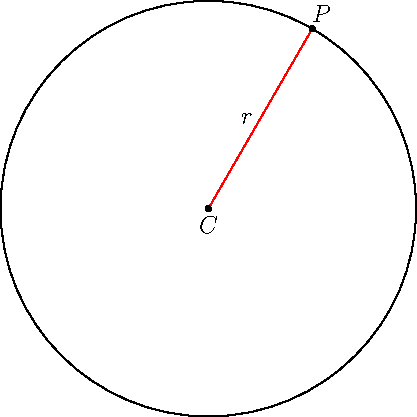
\includegraphics[width=\textwidth,height=1.5in]{fig-circle.pdf} &
		\includegraphics[width=\textwidth,height=1.5in]{fcc.pdf}
	\end{tabular}
	\caption*{A circle schematic, and a circle in a cone}
\end{table}


\textbf{Parent Equation}: The parent equation \(x^2+y^2=1\) is the
equation for the unit circle, a circle centered at the origin with
radius 1.

\textbf{Standard Form Equation}: \((x-h)^2 + (y-k)^2 = r^2\) is a circle
with radius \(r\) centered at \((h,k)\)

\textbf{General Form Equation}: \(Ax^2+Cy^2+Dx+Ey+F=0\). This is the
general form for any (non-rotated) conic.

\textbf{Geometry Review}: Given a line segment joining \((x_1,y_1)\) and
\((x_2,y_2)\)

\begin{itemize}
\tightlist
\item
  the length of the segment is \(\sqrt{(x_2-x_1)^2 + (y_2-y_1)^2}\)
\item
  The midpoint of the segment is
  \(\left(\dfrac{x_1+x_2}{2}, \dfrac{y_1+y_2}{2}\right).\)
\end{itemize}

\textbf{Completing the Square}: You can always rewrite \(x^2 + bx +c\)
as

\begin{itemize}
\tightlist
\item
  \(x^2 + bx +\left(\frac{b}{2}\right)^2 - \left(\frac{b}{2}\right)^2 +c\)
\item
  which is \((x+\frac{b}{2})^2 + (c - \left(\frac{b}{2}\right)^2)\)
\end{itemize}

\hypertarget{problems}{%
\subsection{Problems}\label{problems}}

Unless otherwise specified, any circle equations should be given in
standard form

\hypertarget{fundamental-concepts}{%
\paragraph{Fundamental Concepts}\label{fundamental-concepts}}

\begin{enumerate}
\def\labelenumi{\arabic{enumi}.}
\tightlist
\item
  Find the radius of the circle \(x^2 + y^2 = 100\).
\item
  Find the radius of the circle \(x^2 + y^2 = 72\).
\item
  Find the radius and center of the circle \((x-8)^2 + (y+4)^2 = 20\).
\item
  Translate the circle given here by 5 units up and 3 units to the left:
  \((x+8)^2 + (y+2)^2 = 20\)
\item
  Translate the circle given here so that its center is half as close to
  the origin: \((x+\sqrt{7})^2 + (y + \frac{\sqrt{5}}{2})^2 = \pi\)
\item
  Write the equation of a circle with the same center but half the area
  of the circle \((x-1)^2+(y-5)^2=84\)
\item
  Find the radius and center of the circle
  \((3x-4)^2 = 100 - (3y + 1)^2\)
\item
  Write the equation of a circle with radius 5 and center \((3,-4)\).
  Write both standard and general form.
\item
  Write the equation of a circle with radius \(\frac{\sqrt{17}}{3}\) and
  center \((\frac13,\frac{-2}{3})\). Eliminate all denominators. Write
  both standard and general form.
\item
  A diameter of a certain circle joins the points \((-12,7)\) and
  \((12,14)\). Find the equation of the circle.
\item
  Write the circle \((x+8)^2 + (y - \sqrt2)^2 = 15\sqrt 2\) in general
  form.
\item
  Complete the square to write the following in standard form:
  \(x^2 + 10x + y^2 - 20y - 50 = 0\)
\item
  Complete the square to write the following in standard form:
  \(4x^2 + 8x + 4y^2 - 20y = 100\)
\item
  Write a ``completing the square'' circle problem and trade with a
  friend.
\end{enumerate}

\hypertarget{deeper-understanding}{%
\paragraph{Deeper Understanding}\label{deeper-understanding}}

\begin{enumerate}
\def\labelenumi{\arabic{enumi}.}
\setcounter{enumi}{14}
\tightlist
\item
  An equilateral triangle has its base as the line segment joining the
  points \((-4,-2)\) and \((4,-2)\). Find the third point of the
  triangle. Circumscribe a circle around this triangle and find the
  equation of the circle. (Hint: the center of the circle is the average
  of the three triangle vertices).
\item
  Given the circle \(x^2 + y^2 = 72\), find four points on the circle
  that form the vertices of a square.
\item
  In the general form equation of a circle \(Ax^2+Cy^2+Dx+Ey+F=0\), can
  \(A\) be greater than \(C\)? Can it be less than \(C\)? Why or why
  not?
\item
  Write an inequality which constrains \(F\) in terms of the other
  coefficients in the general form equation of a circle. (Hint: find the
  center and radius of the general equation first by completing the
  square.)
\item
  Find the intersection points of the circle \(x^2 + y^2 = 80\) with the
  line \(y=2x+1\). Round your answer to 3 places.
\item
  A regular hexagon is inscribed in a unit circle. What is its
  perimeter?
\item
  The circle \(x^2 + y^2 = 25\) contains the points \((3,4)\) and
  \((3,-4)\). The tangent line to the circle at the point \((3,4)\) is
  perpendicular to the line segment from the origin to \((3,4)\). Write
  the equation of this tangent line. Also write the equation of the
  tangent line through \((3,-4)\).
\item
  Circle \(C_1\) has radius 1 and is centered at the origin. Circle
  \(C_2\) is tangent to circle \(C_1\) at the point
  \((-\frac{\sqrt2}{2},-\frac{\sqrt2}{2})\), entirely contains circle
  \(C_1\) and has twice the area of \(C_1\). Write the equation of
  \(C_2\) in standard form.
\end{enumerate}

\end{document}
